\section{Newton Polynomial Interpolation}

For some interpolation problem (collocation), a polynomial
$p(x) = c_0 + c_1x + c_2x^2 + \ldots + c_mx^m$
of degree $m$ is required such that the degree $m$ is minimal while meeting collocation condition $y(x_k)=p(x_k)$.

The $n+1$ measurements are given by indexed pairs $(x_k,y_k)$ with $k=0,1,2,\ldots,n$.

\subsection{Aitken-Neville Recursion Formula}

Group together polynomials of a subset of the measurement into a global polynomial, e.g. for a dataset with three measurements:

\begin{align*}
    p_{0,1,2}(x)=\frac{(x-x_0)p_{1,2}(x) - (x-x_2)p_{0,1}(x)}{(x_2-x_0)}
\end{align*}

\subsection{Newton Basis Polynomials}
Given a set $n+1$ of measurements (resulting \emph{order = $n$}).

The basis polynomials with degree $k=0,1,2,\ldots,n$:

\begin{snugshade*}
    \begin{align*}
        \pi_0(x) & = 1 \\
        \pi_1(x) & = (x-x_0) \\
        \pi_2(x) & = (x-x_0)(x-x_1) \\
        \vdots \\
        \pi_n(x) & = (x-x_0)(x-x_1)\cdots(x-x_{n-1})
    \end{align*}
\end{snugshade*}

can be used to form a collocation polynomial using a linear combination
$p(x)=a_0\pi_0(x) + a_1\pi_1(x) + \ldots + a_m\pi_m(x)$.
This forms the system of linear equations
\begin{align*}
    y_0 & = a_0 \\
    y_1 & = a_0 + a_1(x_1-x_0) \\
    y_2 & = a_0 + a_1(x_2-x_0) + a_2(x_2-x_0)(x_2-x_1) \\
    \vdots \\
    y_n & = a_0+a_1\pi_1(x_n)+a_2\pi_2(x_n)+\ldots+a_n\pi_n(x_n)
\end{align*}

\emph{Stability}: Since the coefficient $a_k$ is determined by the first $k$ arguments,
we can extend the dataset with new data without altering existing coefficients.

\subsubsection{Divided Differences}

Due to stability, we can write the coefficients as $a_k(x_0,\ldots,x_k)$, only depending on the arguments lower than $k$.
Applying the Aitken-Neville formula, we receive for $k=0,1,\ldots,n$:

\begin{align*}
    y(x_0, x_2, \ldots, x_k)=\frac{y(x_1,x_2,\ldots,x_k) - y(x_0, x_1, \ldots, x_{k-1})}{(x_k - x_0)}
\end{align*}

\makebox[\columnwidth]{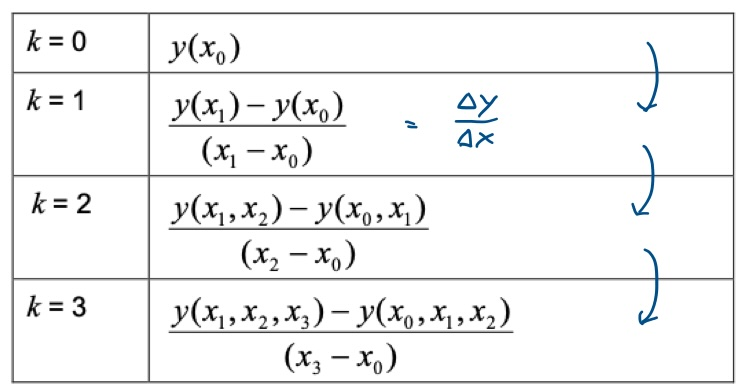
\includegraphics[width=0.6\columnwidth]{images/aitken-neville}}

\makebox[\columnwidth]{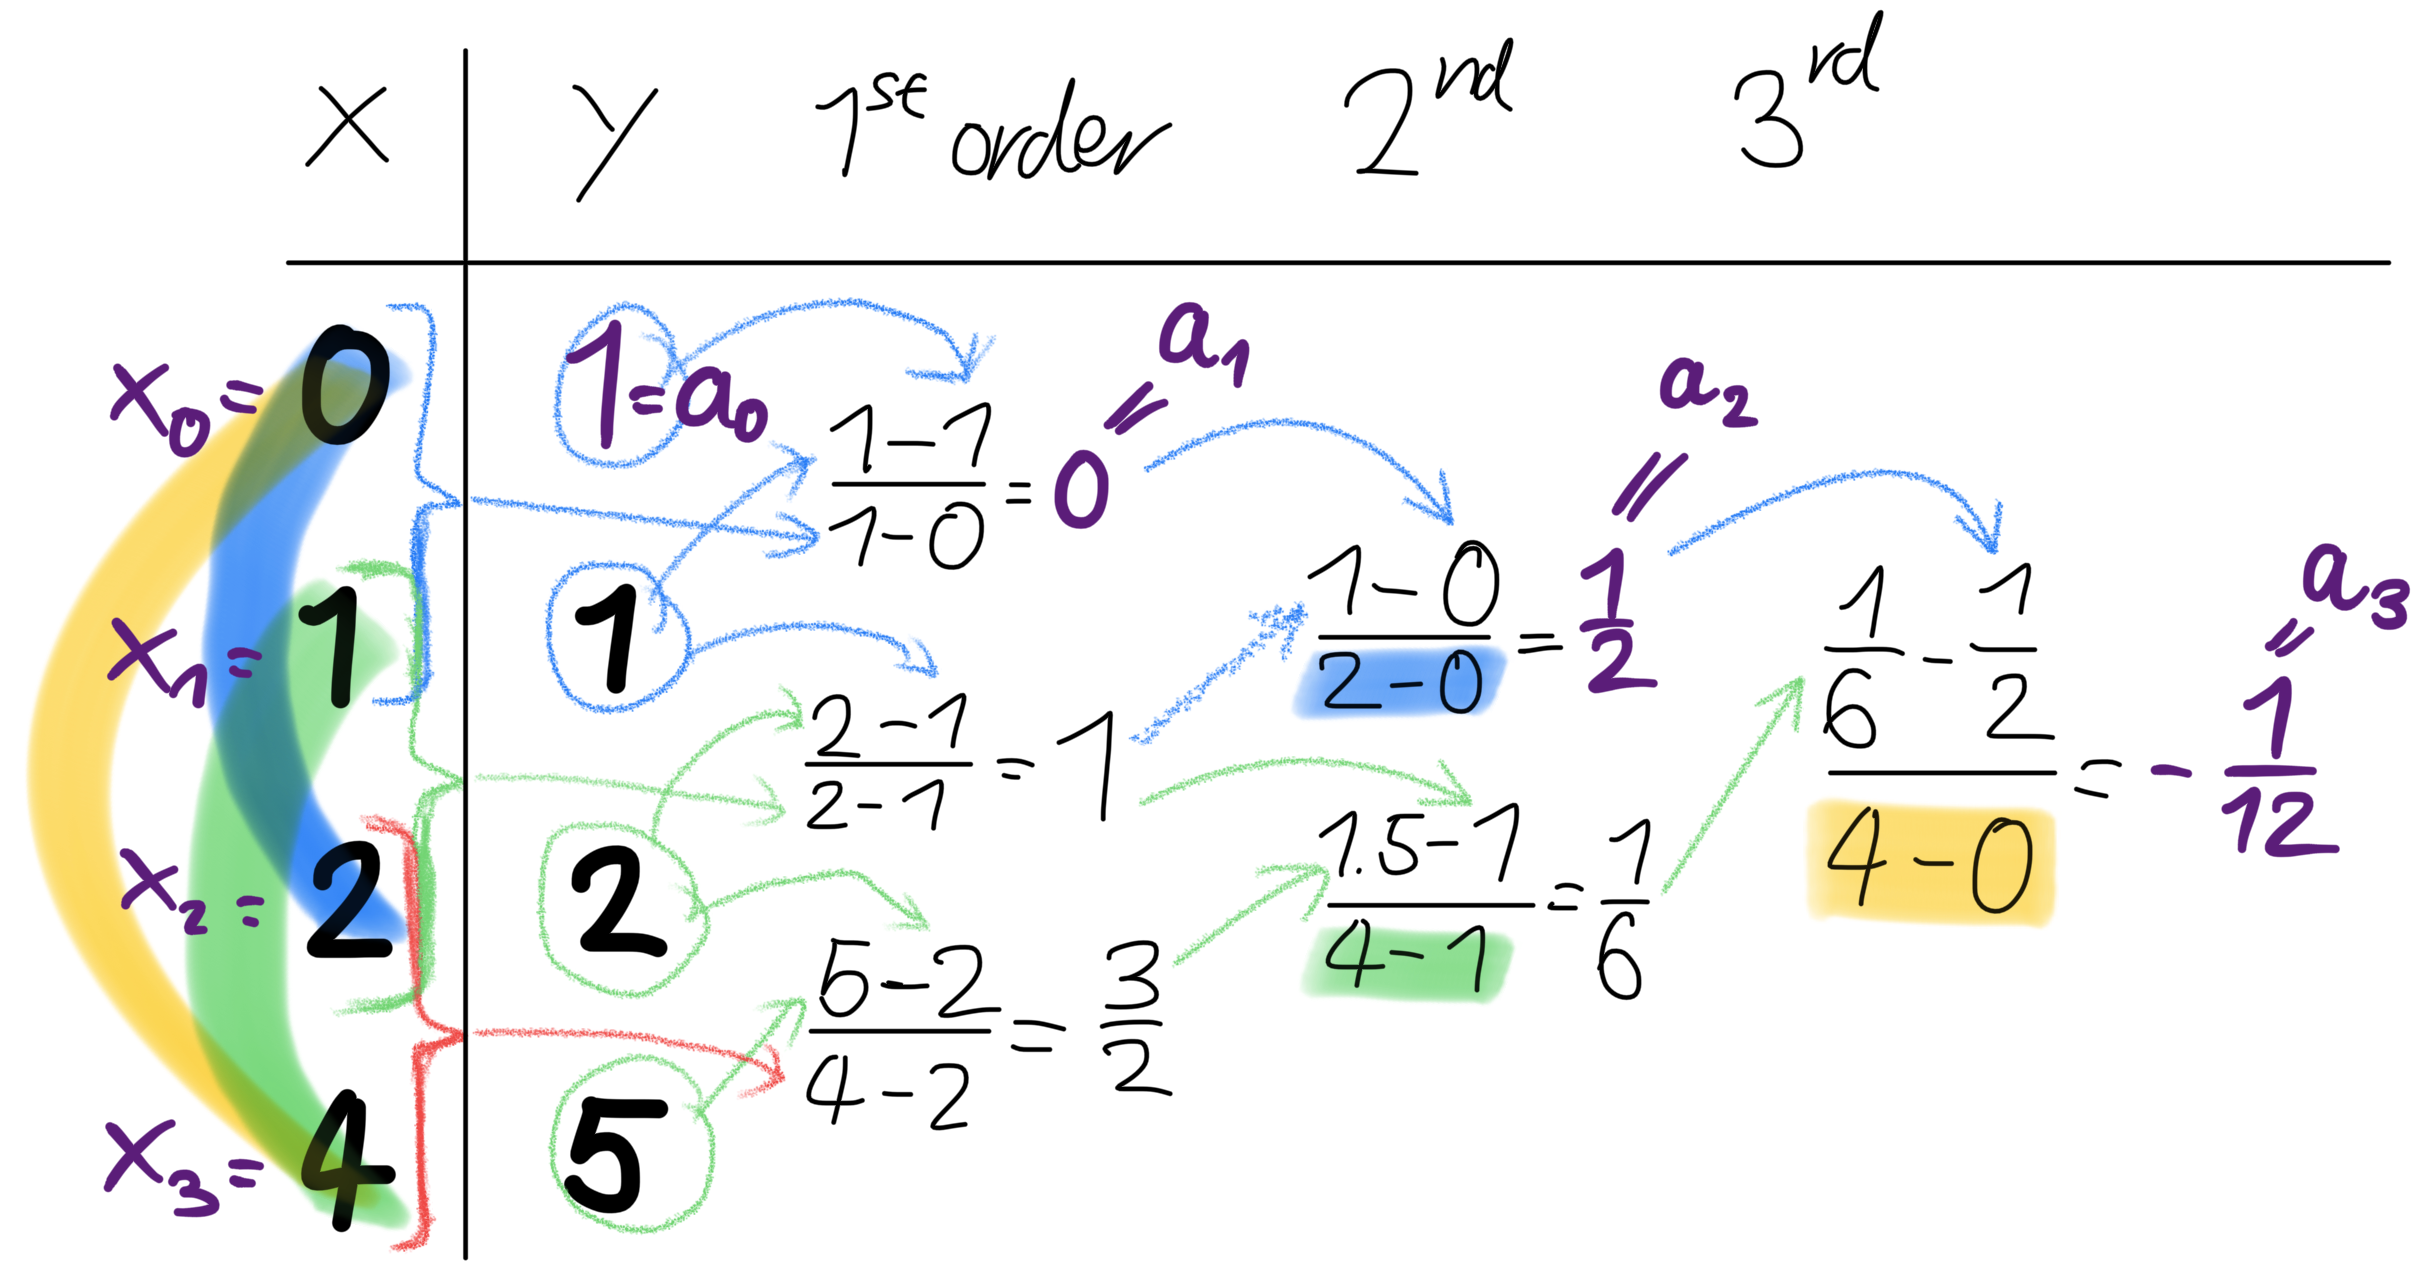
\includegraphics[width=0.6\columnwidth]{images/divided-differences}}

from which (in this special example above) we can derive the collocation polynomial
\begin{align*}
    y(x)=p(x)={\color{purple}1} + {\color{purple}0}\cdot\pi_1(x) + {\color{purple}0.5}\cdot\pi_2(x)
    - {\color{purple}\frac{1}{12}}\pi_3(x)
\end{align*}

\subsubsection{Error Formula}

With the ``real'', physical (usually unknown) function $y=f(x)$ interpolated by $p(x)$ and some intermediate value $\xi$:
\begin{align*}
    & \varepsilon = |y(x)-p(x)| = \left|\frac{f^{(n+1)}(\xi)}{(n+1)!}\pi_{n+1}(x)\right| \\
    & \left[\xi\in \left(\min(x_k),\max(x_k)\right) ,x\in (\min(x_k),\max(x_k))\right]
\end{align*}

With large values of $n$, this leads to the \emph{Runge phenomenon} (oscillation of errors towards the boundaries of arguments range),
mainly because one can interpret divided differences as derivations.

\subsubsection{Chebyshev Arguments for the Runge Phenomenon}

Choosing the Chebyshev arguments

\begin{align*}
    x_k = \cos\left( \frac{2k+1}{2(n+1)}\pi \right)\ (k=0,1,\ldots,n)
\end{align*}

in the interval $[-1,1]$ minimises the maximum amplitude to $2^{-n}$:

\begin{align*}
    \min_{\{x_0,x_1,\ldots,x_n\}}\max_{-1\leq x \leq 1} \left|\pi_{n+1}(x)\right| \leq \frac{1}{2^n}
\end{align*}

We therefore need the affine formula $x\rightarrowtail a+\frac{b-a}{2}(x+1)$
to transform the interval $[-1,1]$ into $[a,b]$ in which our measurement x-values reside.
Downsides: Expense of increased measurements at edges of the interval.
Also, increasing the number of $n$ (meas.\ minus 1) implies that nearly all arguments and Newton basis polynomials change.

\subsubsection{Uniformly distributed arguments}

For uniformly distributed arguments, where $h$ is the step size ($x_k = x_0 + kh$),
the polynomial $p$ is given by
\begin{align*}
    p(x) = \sum_{k=0}^n \frac{\Delta^k y_0}{h^kk!}\pi_k(x)
\end{align*}

with $\Delta$ as difference operator $\Delta y_k=y_{k+1} - y_k$
and $\Delta^m$ for the composition (e.g. $\Delta^2 = \Delta y_1 - \Delta y_0 = (y_2-y_1) - (y_1-y_0)$).

\subsubsection{Taylor-Approximation}

With a model function $y=f(x)$ with continuous derivatives up to order $n$ on the interval $[x_0,x]$:
\begin{align*}
    p(x) & = y_0 + \frac{y'(x_0)}{1!}(x-x_0) + \frac{y''(x_0)}{2!}(x-x_0)^2 + \\
    \ & \ldots + \frac{f^{(n)}(x_0)}{n!}(x-x_0)^n {\color{blue} \underbrace{+ \frac{f^{(n+1)}(\xi)}{(n+1)!}(x-x_0)^{n+1}}_{\text{Lagrange error term}}}
\end{align*}
